\documentclass[11pt]{cernrep}
\usepackage{graphicx,epsfig}
\bibliographystyle{lesHouches}

\usepackage{xspace}
\newcommand{\Sherpa}{S\protect\scalebox{0.8}{HERPA}\xspace}
\newcommand{\Powheg}{P\protect\scalebox{0.8}{OWHEG}\xspace}
\newcommand{\CSS}{C\protect\scalebox{0.8}{SS}\xspace}
\newcommand{\Comix}{C\protect\scalebox{0.8}{OMIX}\xspace}
\newcommand{\Amegic}{A\protect\scalebox{0.8}{MEGIC++}\xspace}
\newcommand{\MCatNLO}{M\protect\scalebox{0.8}{C}@N\protect\scalebox{0.8}{LO}\xspace}
\newcommand{\MEPS}{M\scalebox{0.8}{E}P\scalebox{0.8}{S}\xspace}
\newcommand{\MEPSatNLO}{M\scalebox{0.8}{E}P\scalebox{0.8}{S}@N\protect\scalebox{0.8}{LO}\xspace}
\newcommand{\Collier}{C\protect\scalebox{0.8}{OLLIER}\xspace}
\newcommand{\OpenLoops}{O\protect\scalebox{0.8}{PEN}L\protect\scalebox{0.8}{OOPS}\xspace}
\newcommand{\Herwig}{H\protect\scalebox{0.8}{ERWIG}7\xspace}
\newcommand{\Matchbox}{M\protect\scalebox{0.8}{ATCHBOX}\xspace}
\newcommand{\MGaMC}{M\protect\scalebox{0.8}{AD}G\protect\scalebox{0.8}{RAPH}5\_aMC@NLO\xspace}
\newcommand{\MadGraph}{M\protect\scalebox{0.8}{AD}G\protect\scalebox{0.8}{RAPH}\xspace}
\newcommand{\MadGraphfour}{M\protect\scalebox{0.8}{AD}G\protect\scalebox{0.8}{RAPH}4\xspace}
\newcommand{\CVolver}{CV\protect\scalebox{0.8}{OLVER}\xspace}
\newcommand{\ColorFull}{C\protect\scalebox{0.8}{OLOR}F\protect\scalebox{0.8}{ULL}\xspace}
\newcommand{\MoCaNLO}{M\protect\scalebox{0.8}{oCaNLO}\xspace}
\newcommand{\Recola}{R\protect\scalebox{0.8}{ecola}\xspace}
\newcommand{\pt}{\ensuremath{p_{T}}\xspace}
\newcommand\sss{\mathchoice%
{\displaystyle}%
{\scriptstyle}%
{\scriptscriptstyle}%
{\scriptscriptstyle}%
}
\newcommand\MSB{\ifmmode {\overline{\rm MS}} \else $\overline{\rm MS}$\fi}
\newcommand\MINLO{{\tt MiNLO}}
\newcommand\muf{\mu_{\sss\rm F}}
\newcommand\mur{\mu_{\sss\rm R}}
\newcommand\KRA{K_{\scriptscriptstyle \rm R}}
\newcommand\KFA{K_{\scriptscriptstyle \rm F}}

\newcommand{\GOSAM}{G\protect\scalebox{0.8}{O}S\protect\scalebox{0.8}{AM}\xspace}
\newcommand{\POWHEGBOX}{P\protect\scalebox{0.8}{OWHEG} B\protect\scalebox{0.8}{OX}\xspace}
\newcommand{\QGRAF}{Q\protect\scalebox{0.8}{GRAF}\xspace}
\newcommand{\FORM}{F\protect\scalebox{0.8}{ORM}\xspace}
\newcommand{\SAMURAI}{S\protect\scalebox{0.8}{AMURAI}\xspace}
\newcommand{\GOLEM}{G\protect\scalebox{0.8}{OLEM}\xspace}
\newcommand{\NINJA}{N\protect\scalebox{0.8}{INJA}\xspace}
\newcommand{\SPINNEY}{S\protect\scalebox{0.8}{PINNEY}\xspace}
\newcommand{\ONELOOP}{O\protect\scalebox{0.8}{NE}LO\protect\scalebox{0.8}{OP}\xspace}
\newcommand{\MCFM}{M\protect\scalebox{0.8}{CFM}\xspace}


\newcommand{\MP}[1]{{ {\color{blue}{ [MP: #1]}} }}

\usepackage{color}
\usepackage{morefloats}

\begin{document}

\section{Study of electroweak production of WZ in association with two
  jets at the LHC \protect\footnote{Section
    coordinators: K.~D.~Long, M.~Pellen}$^{,}$ \protect\footnote{Contributing authors:
    S.~Br\"auer, V.~Ciulli, M.~Herndon, S.~Gieseke, S.~Pl{\"a}tzer,
    M.~Rauch, E.~Yazgan,...}$^{,}$
  \protect\footnote{{\it next some examples of acknowledgements}}$^{,}$
  \protect\footnote{ A. Aaaaa acknowledges support by a FP7 Marie
    Curie Intra European Fellowship under Grant Agreement xxxx.}$^{,}$
\protect\footnote{The work of B. Bbbb is supported in part by the
  U.S. Department of Energy under grant yyyy.} \label{vbs_section}}

\subsection{Introduction \label{vbs_intro}}

The electroweak production of vector boson pairs in association with two jets at the
CERN Large Hadron Collider (LHC) is important for many different experimental and
theoretical reasons. 
From the theoretical point of view, it is the first process when one can observe the scattering of two gauge bosons.
In the scattering of two massive gauge bosons, the Higgs boson is playing a very special role.
It prevents the cross section from diverging in the high energy limit and preserve the unitarity of the associated scattering amplitude.
More importantly, these vector-boson scattering (VBS) signatures just started to be observed and even measured by the experimental collaborations at the LHC.
The best measurement concern the signature with the scattering of same sign W boson \cite{Aad:2014zda,Khachatryan:2014sta,Sirunyan:2017ret,Aaboud:2016ffv}.
The reason for this is that is posses a very specific structure due to the same sign charged leptons.
Therefore, in addition to have a rather large cross section, it also possesses a low irreducible background.
Other signature such as ZZ or WZ are more challenging due to the lower cross section and large irreducible background \MP{Experimental references to be added.}.
Nonetheless, observations have already been performed at the LHC.

Some extra comments on the specific experimental challenge to measure WZ.
Therefore a preliminary study aiming at comparing various approximation used in the literature is particularly well motivated.
The present study focus on LO predictions (possibly supplied with a parton shower) with realistic experimental event selection.

\subsection{Theory and event generators \label{vbs_theory}}

Even if this study focus on LO prediction, NLO corrections to the EW contribution and its irreducible background are already known.
The QCD corrections to the EW contributions are know since XX in the VBS approximation \MP{Add references.}.
The QCD irreducible background is also know \MP{Add references.}.
EW corrections are still currently unknown.
In Refs.~\cite{Biedermann:2016yds}, it has been argued that large NLO EW corrections to the EW contributions are an intrinsic feature of VBS at the LHC.
Therefore, it is expected to also play a significant role for all VBS signatures.
In Ref.~\cite{Biedermann:2017bss}, which focus on the computation of the full NLO corrections to W+W+, it has been shown that the EW corrections to the EW contribution are the dominant NLO corrections.

{\it Add here a description of the theory tools and generators
  used. Below there are same short samples taken from previous proceedings.}

\subsubsection*{\Herwig \label{vbs_herwig}}

In this section we present the setup for those results obtained with the
\Herwig event generator~\cite{Bellm:2015jjp,Bahr:2008pv}.

Based on extensions of the previously developed \Matchbox
module~\cite{Platzer:2011bc}, \Herwig facilitates the automated setup of all
ingredients necessary for a full NLO QCD calculation in the subtraction
formalism: an implementation of the Catani--Seymour dipole subtraction
method~\cite{Catani:1996vz,Catani:2002hc}, as well as interfaces to a list of
external matrix--element providers -- either at the level of squared matrix
elements, based on extensions of the BLHA
standard~\cite{Binoth:2010xt,Alioli:2013nda,Andersen:2014efa}, or at the
level of color--ordered subamplitudes, where the color bases are provided by
an interface to the \ColorFull~\cite{Sjodahl:2014opa} and
\CVolver~\cite{Platzer:2013fha} libraries.

For this study the relevant tree--level matrix elements etc, etc... 

The PDF sets being used are MMHT2014lo68cl and
MMHT2014nlo68cl~\cite{Harland-Lang:2014zoa}, i.e. the default PDF sets
to which the showers are currently tuned.

\subsubsection*{\protect\Sherpa \label{vbs_sherpa}}
In this section we present the setups that are used in this study for the \Sherpa event
generator~\cite{Gleisberg:2008ta}. 
Etc, etc... 

\subsubsection*{\protect{\MoCaNLO+\Recola} \label{vbs_MoCaNLO_Recola}}

The program {\sc MoCaNLO+Recola} is made of a flexible Monte Carlo program dubbed {\sc MoCaNLO} and of the general matrix element generator {\sc Recola}~\cite{Actis:2012qn,Actis:2016mpe}.
The fast integration is ensured by using similar phase-space mappings to those of Refs.~\cite{Berends:1994pv,Denner:1999gp,Dittmaier:2002ap}.
The IR divergences appearing in the real corrections are handles with the help of the Catani--Seymour dipole formalism \cite{Catani:1996vz,Dittmaier:1999mb}.
To numerically evaluate the one-loop scalar and tensor integrals, {\sc Recola} relies on the {\sc Collier} library \cite{Denner:2014gla,Denner:2016kdg}.
These tools have been successfully used for the computation of NLO corrections for high-multiplicity processes and in particular VBS~\cite{Biedermann:2016yds,Biedermann:2017bss}.

\subsection{Experimental analysis \label{vbs_rivet}}

Results in this study were produced using a Rivet routine that
mimics ATLAS and CMS preliminary analyses. Distributions include the number of jets, etc,...

\subsubsection*{Event selection}

\subsubsection*{Input parameters}

\subsection{Results \label{vbs_results}}

The plot in Figure~\ref{vbs_fig1} etc... 

\begin{figure}[htbp]
\begin{center}
   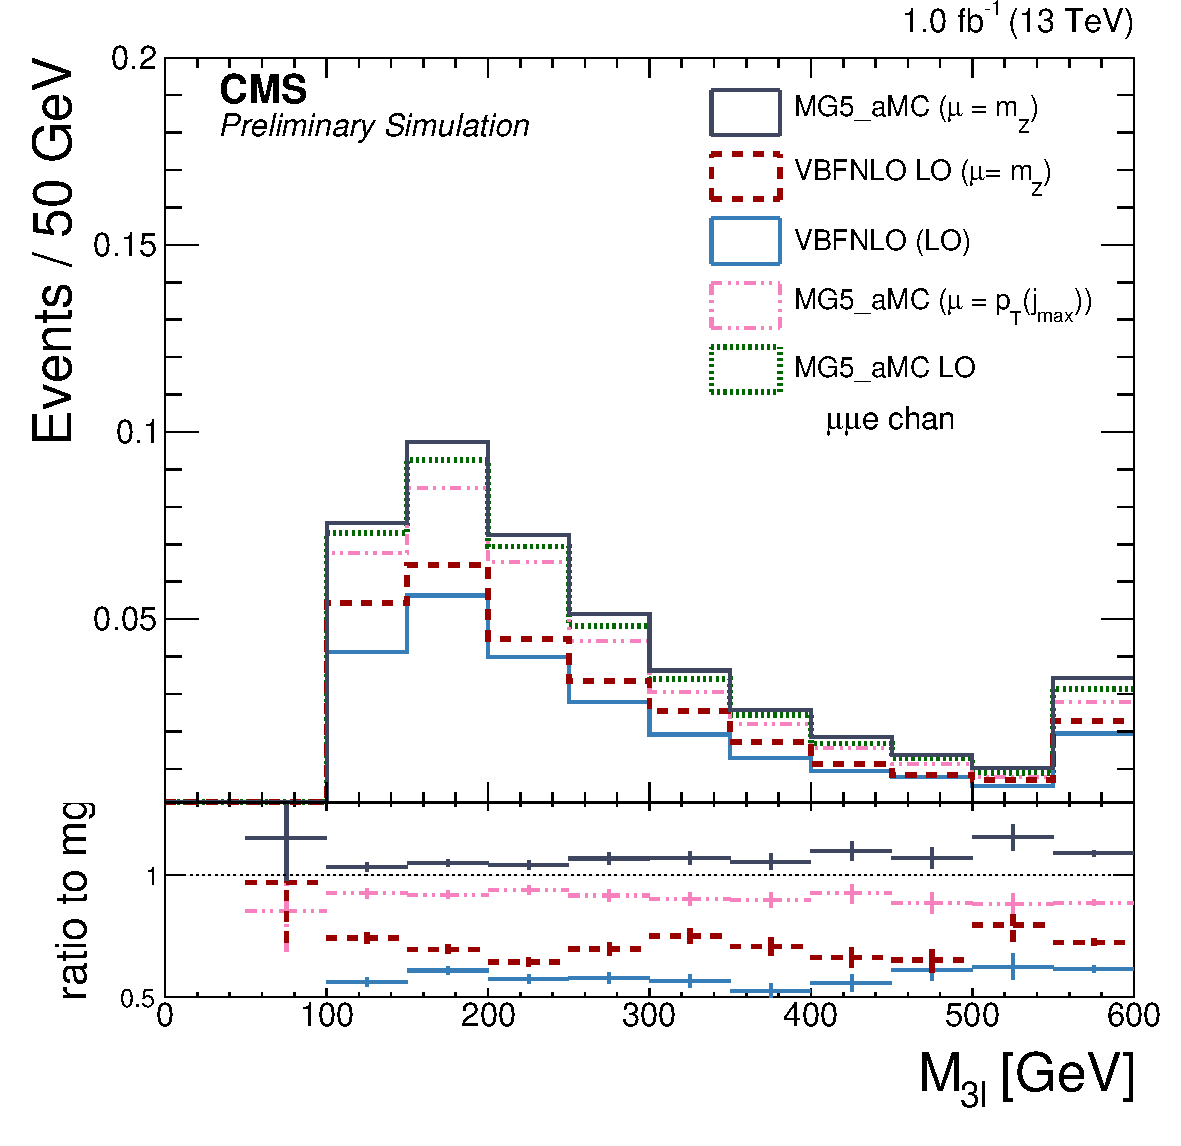
\includegraphics[scale=0.65]{figs/3lmass.pdf}
\caption{A placeholder...}
\label{vbs_fig1}
\end{center}
\end{figure}

\subsection{Conclusions \label{concl}}

We presented a comparison of generators predictions for the

electroweak production of WZ in association with two jets at the LHC, etc... 

Overall these results show that etc...

%\clearpage
\bibliography{vbs_bib}

\end{document}
